\section{Experimental Results}

First we observe the top-1 and top-5 validation-error evolution of the
four variants during training. After the experiment was conducted, we have
found that our continuous evaluation was conducted on a subset of the
validation set which omitted about 1700 blacklisted entities due to poor
bounding boxes. It turned out that the omission should have been only performed
for the CLSLOC benchmark, but yields somewhat incomparable (more optimistic)
numbers when compared to other reports including some earlier reports by our
team. The difference is about 0.3\% for top-$1$ error and about 0.15\% for
the top-$5$ error. However, since the differences are consistent, we think
the comparison between the curves is a fair one.

On the other hand, we have rerun our multi-crop and ensemble results on the
complete validation set consisting of 50000 images. Also the final ensemble
result was also performed on the test set and sent to the ILSVRC test server
for validation to verify that our tuning did not result in an over-fitting.
We would like to stress that this final validation was done only once and we
have submitted our results only twice in the last year: once for the
BN-Inception paper and later during the ILSVR-2015 CLSLOC competition, so
we believe that the test set numbers constitute a true estimate of the
generalization capabilities of our model.

\begin{figure}
\centering
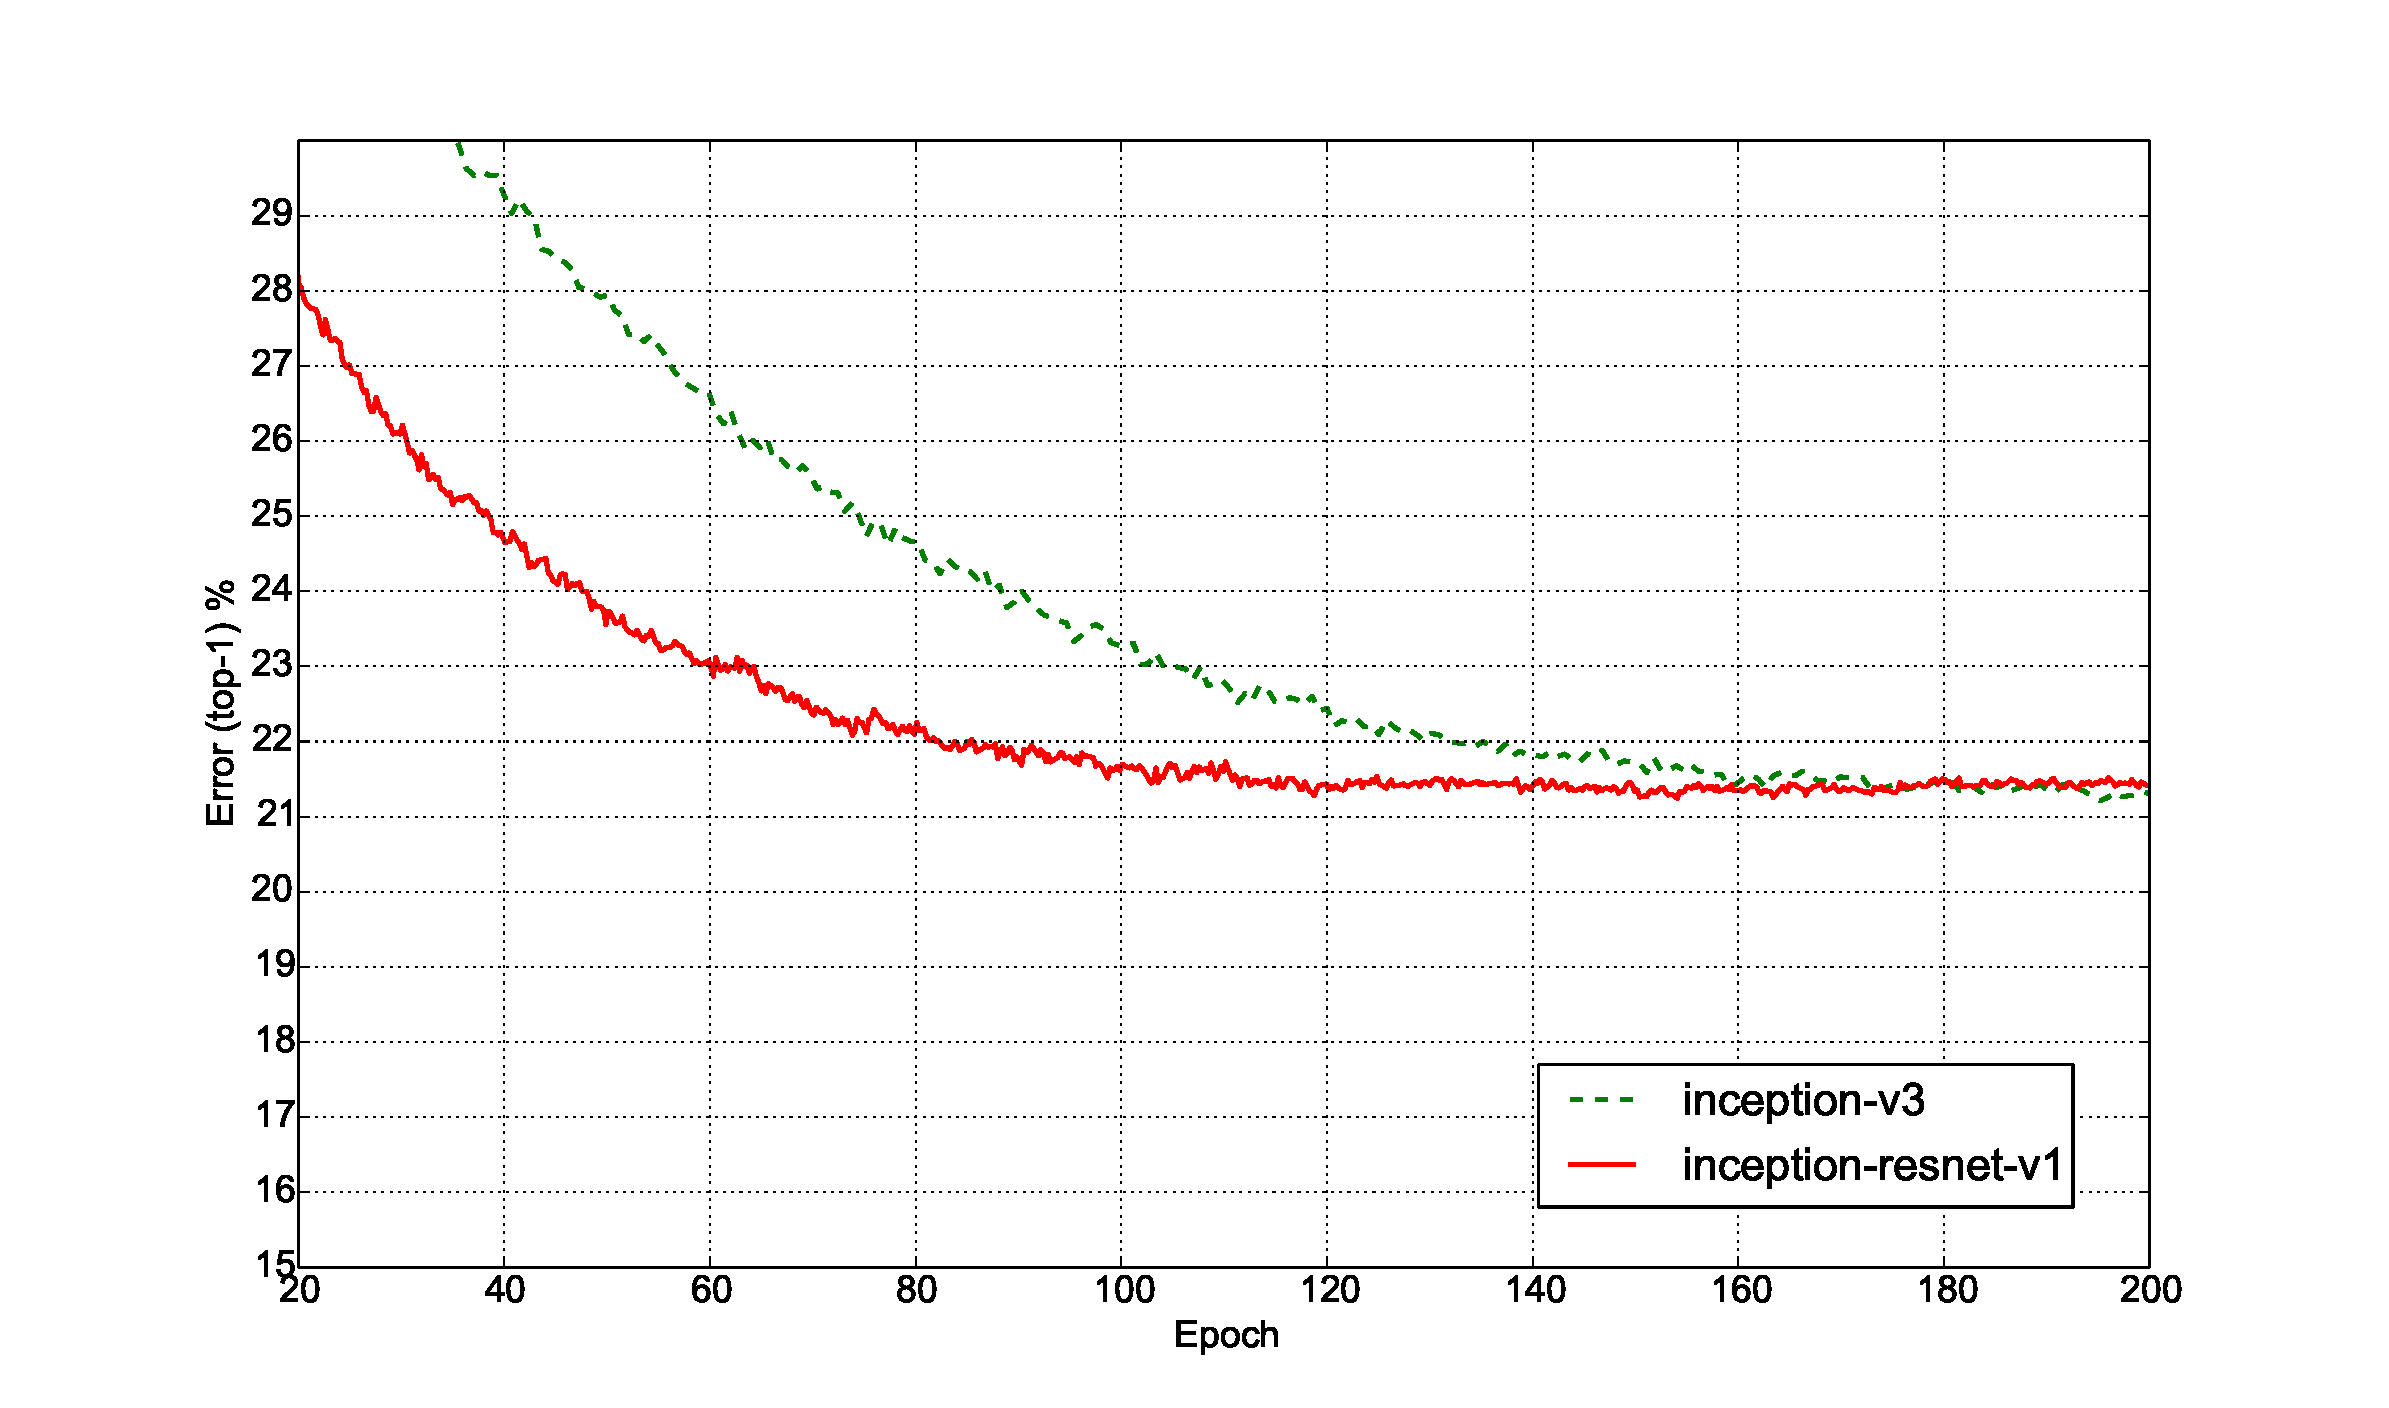
\includegraphics[width=\linewidth]{small_top1}
\caption{Top-1 error evolution during training of pure Inception-v3 vs a
  residual network of similar computational cost. The evaluation is measured on
  a single crop on the non-blacklist images of the ILSVRC-2012 validation set.
  The residual model was training much faster, but reached
  slightly worse final accuracy than the traditional Inception-v3.
}
\label{fig:smalltop1}
\end{figure}

\begin{figure}
\centering
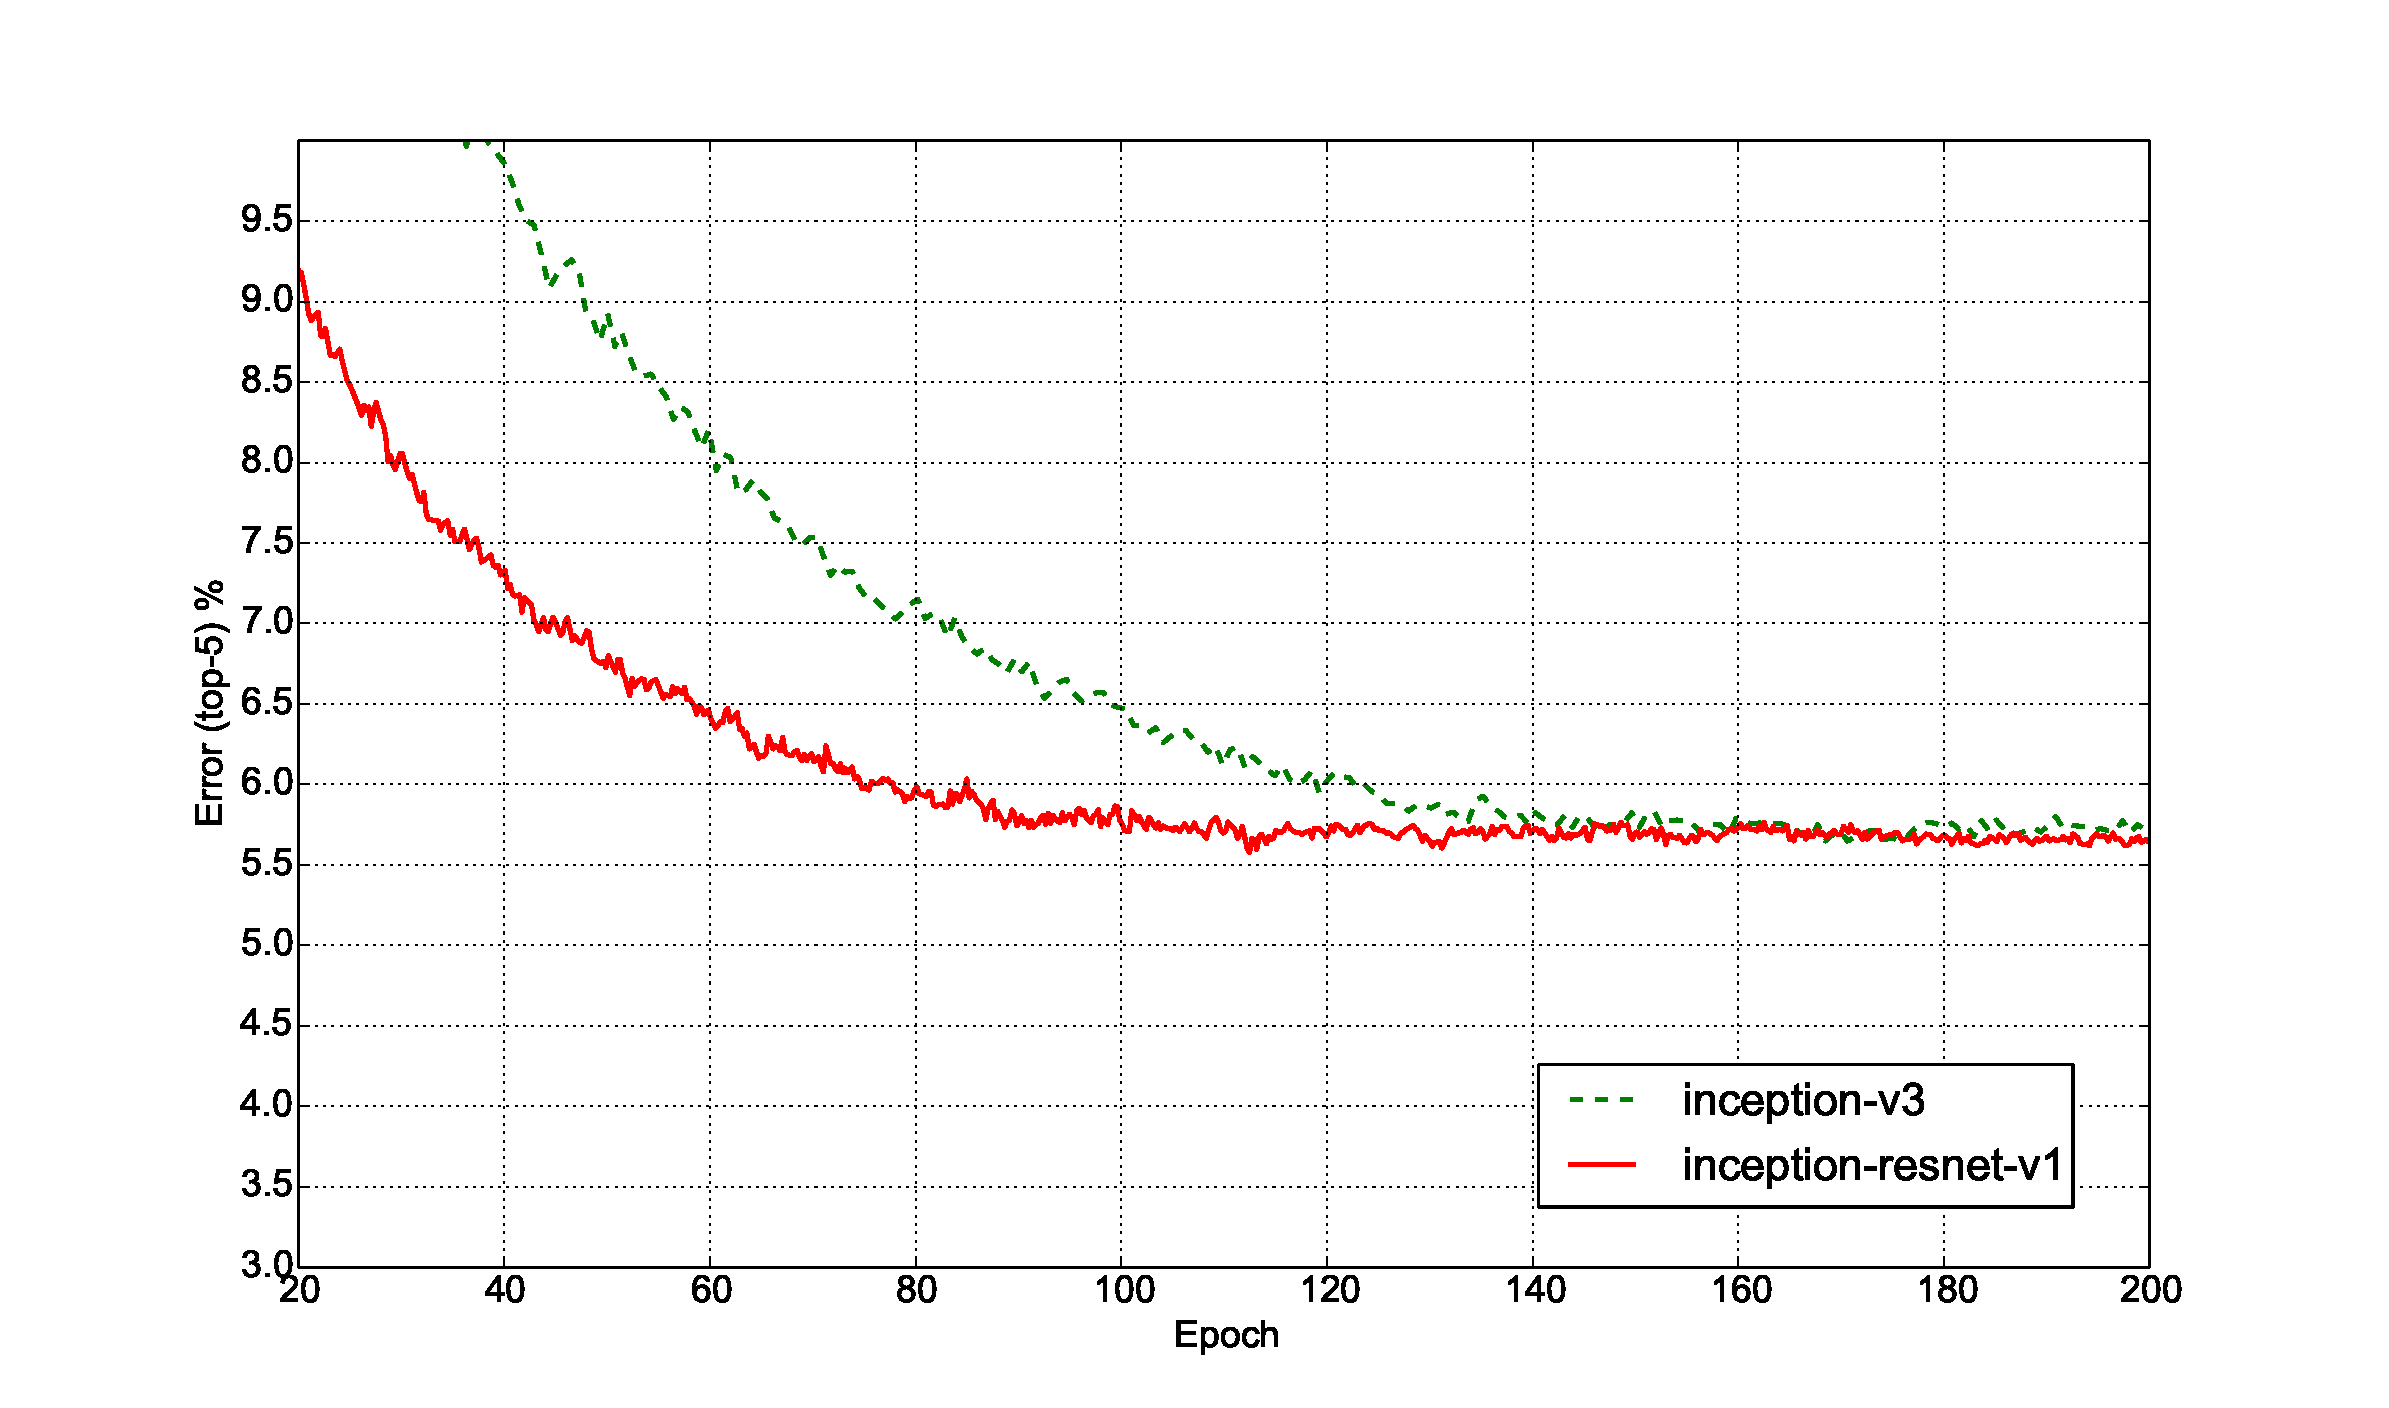
\includegraphics[width=\linewidth]{small_top5}
\caption{Top-5 error evolution during training of pure Inception-v3 vs a
  residual Inception of similar computational cost. The evaluation is measured on
  a single crop on the non-blacklist images of the ILSVRC-2012 validation set.
  The residual version has trained much faster and reached slightly better final recall
  on the validation set.
}
\label{fig:smalltop5}
\end{figure}


\begin{figure}
\centering
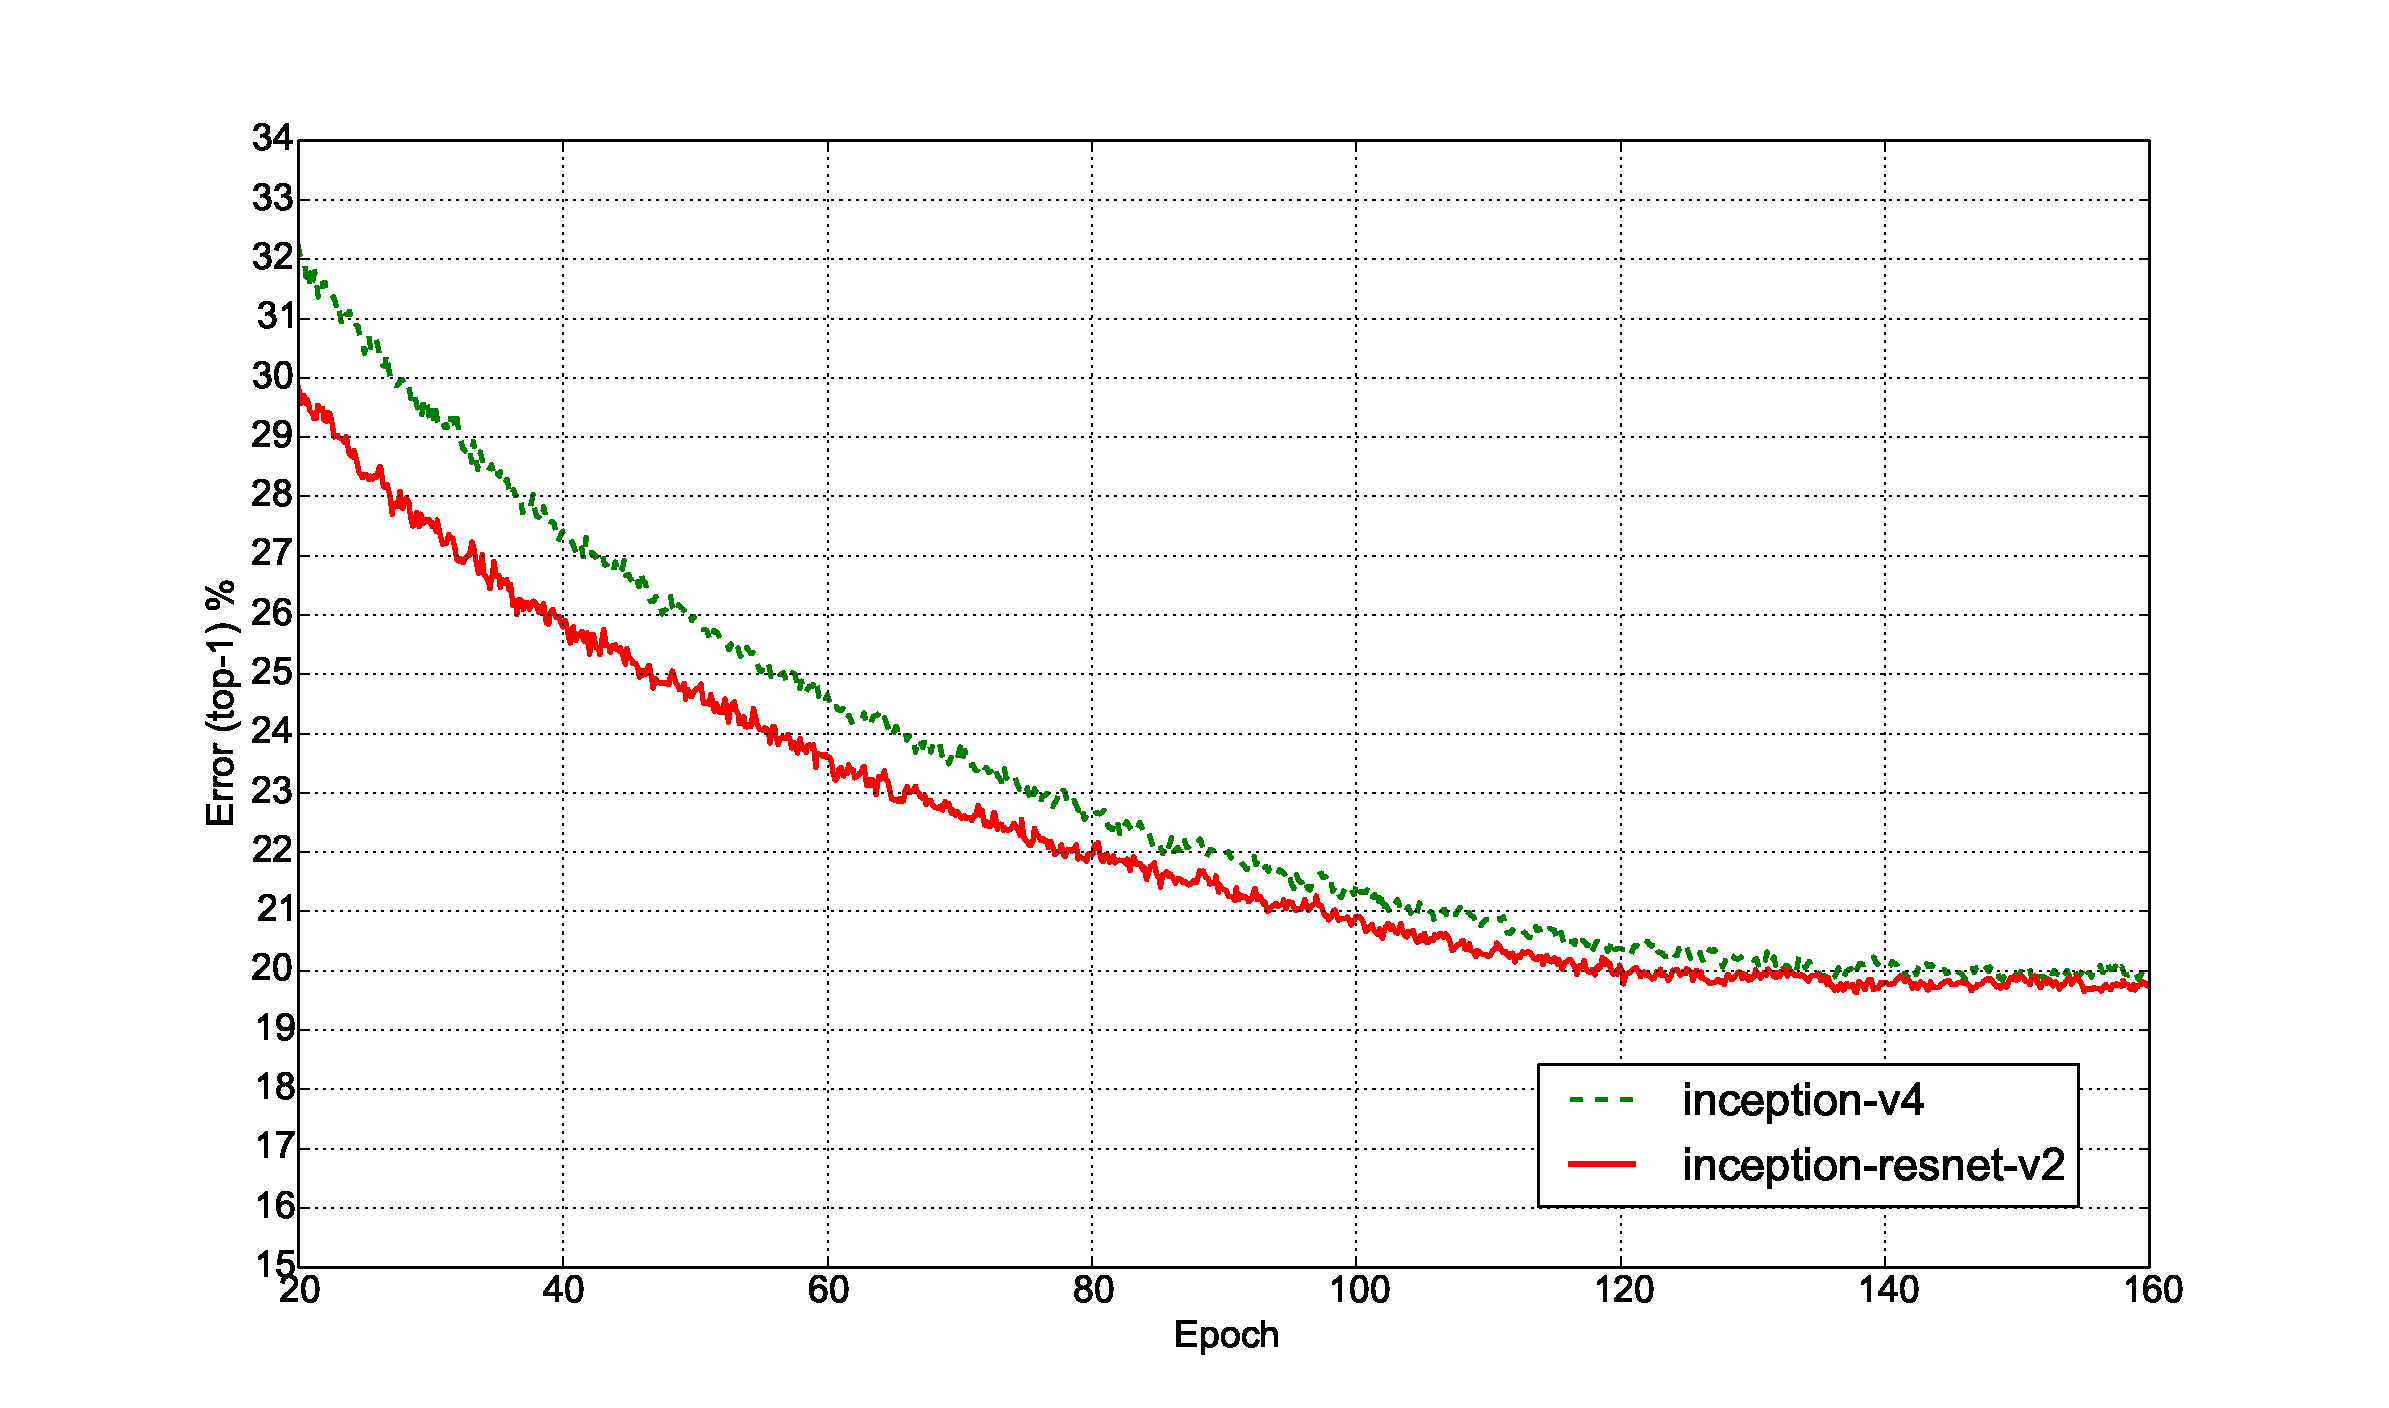
\includegraphics[width=\linewidth]{wide_top1}
\caption{Top-1 error evolution during training of pure Inception-v3 vs a
  residual Inception of similar computational cost. The evaluation is measured on
  a single crop on the non-blacklist images of the ILSVRC-2012 validation set.
  The residual version was training much faster and reached
  slightly better final accuracy than the traditional Inception-v4.
}
\label{fig:widetop1}
\end{figure}

\begin{figure}
\centering
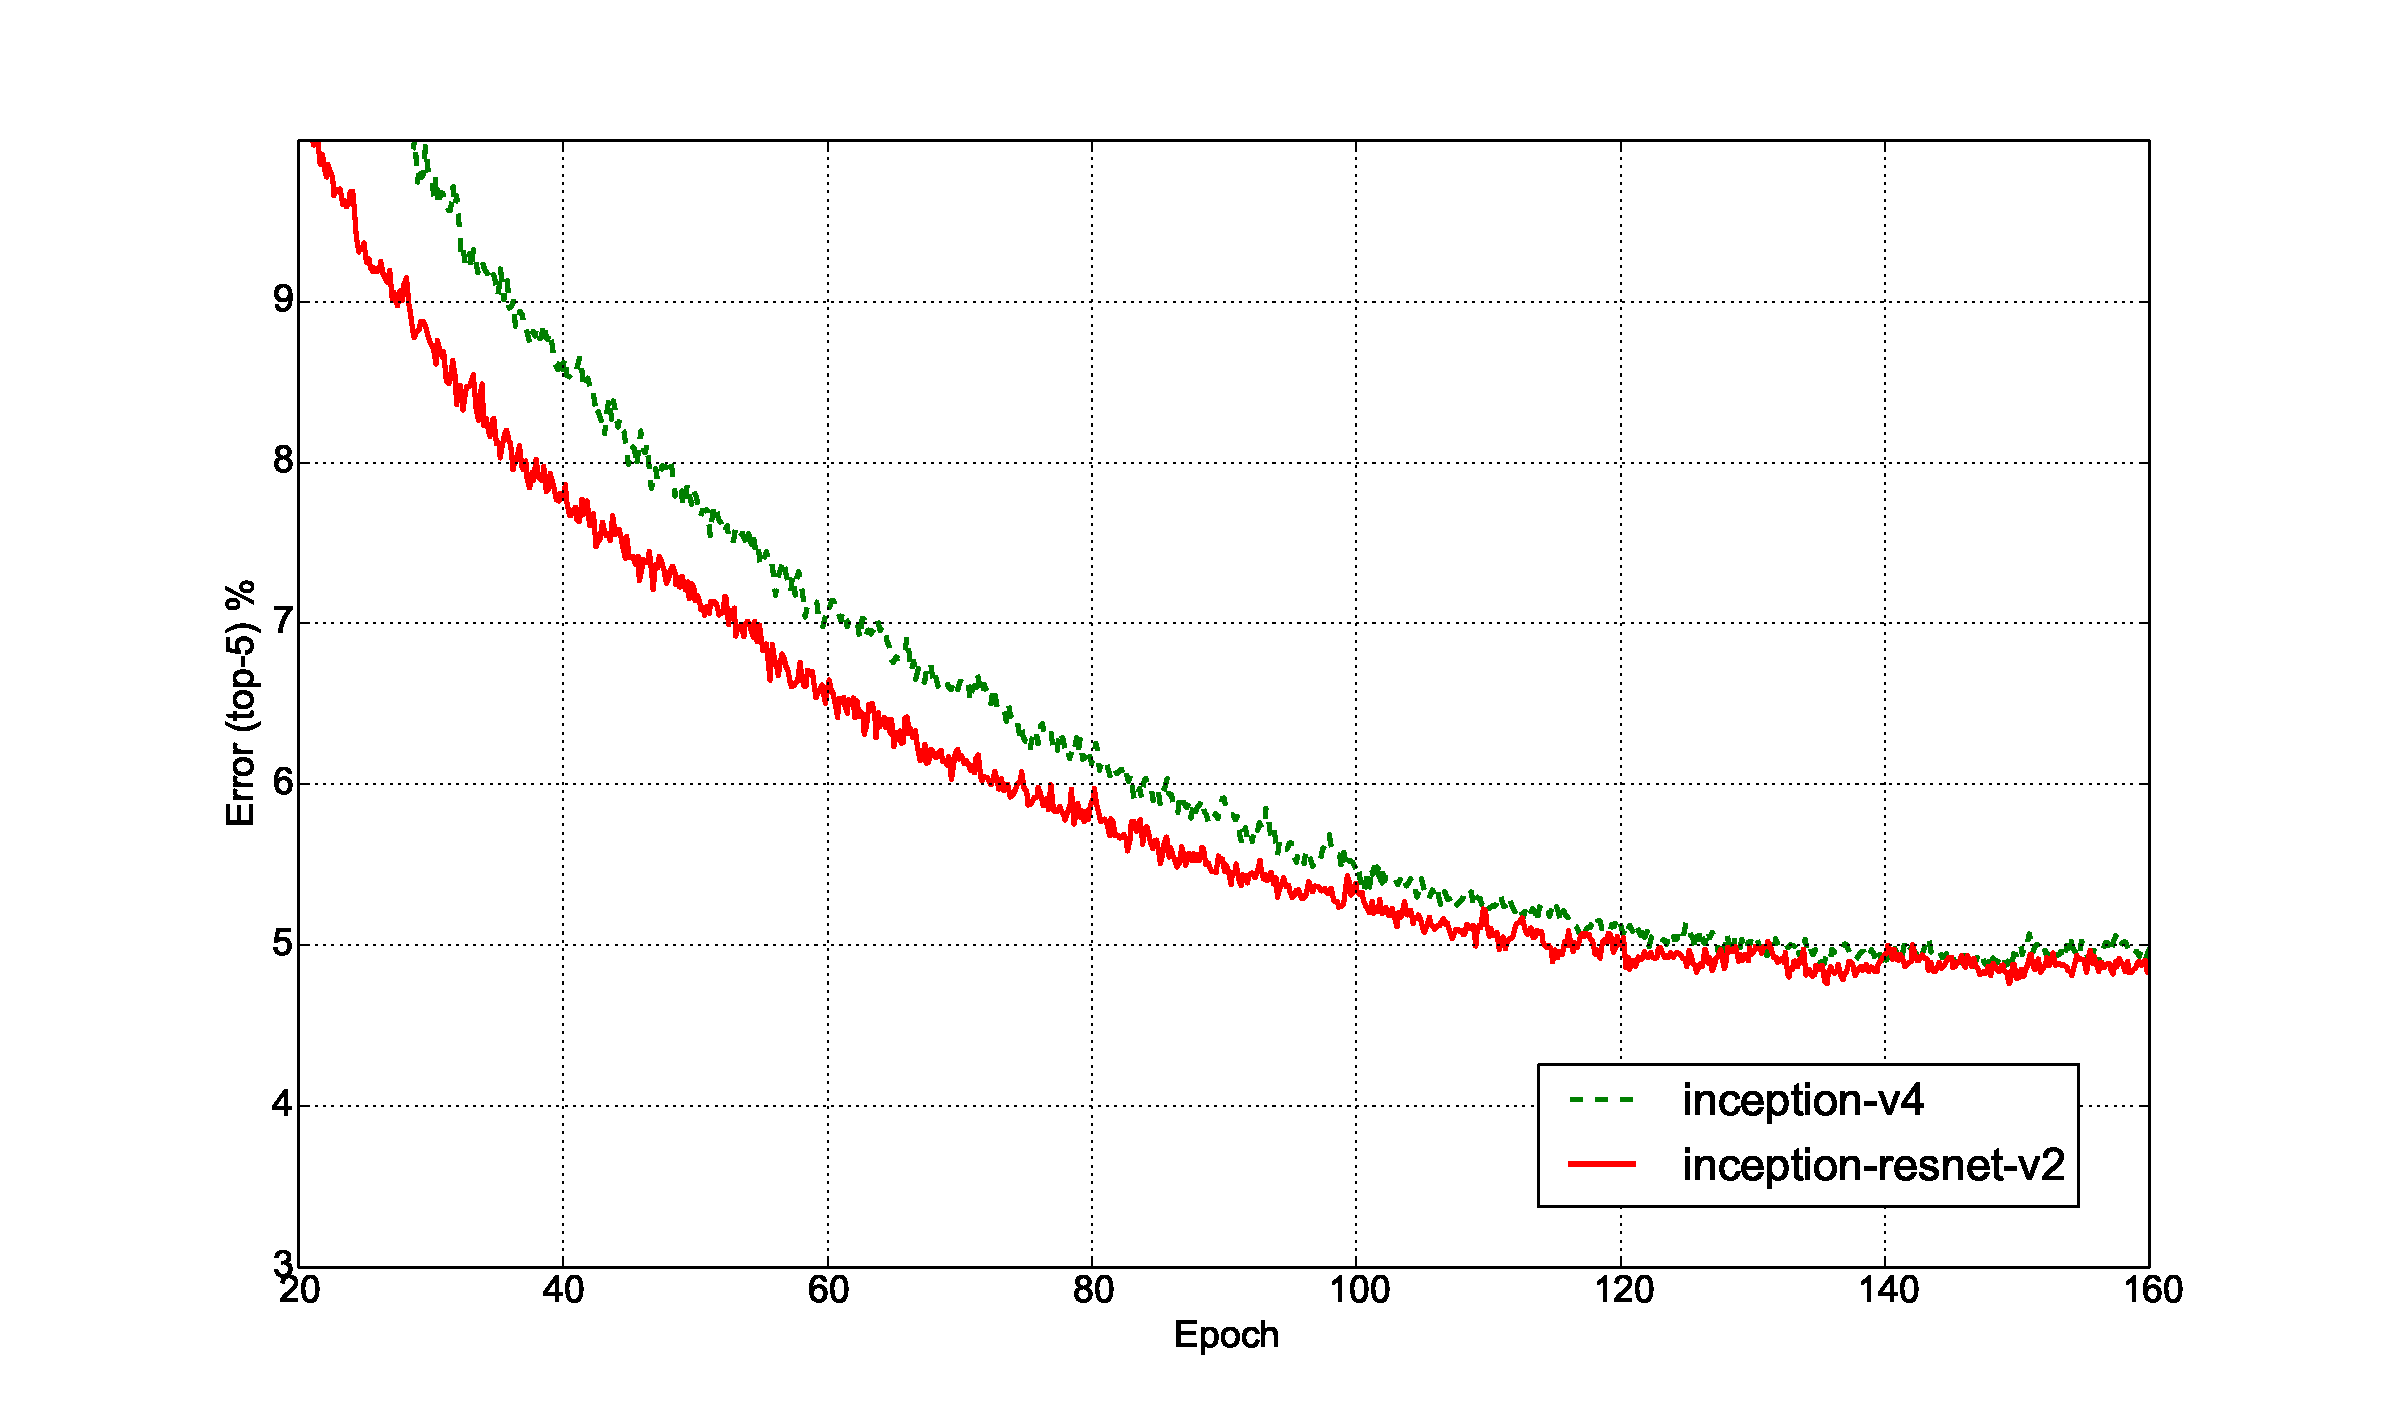
\includegraphics[width=\linewidth]{wide_top5}
\caption{Top-5 error evolution during training of pure Inception-v4 vs a
  residual Inception of similar computational cost. The evaluation is measured on
  a single crop on the non-blacklist images of the ILSVRC-2012 validation set.
  The residual version trained faster and reached slightly better final recall
  on the validation set.
}
\label{fig:widetop5}
\end{figure}

\begin{figure}
\centering
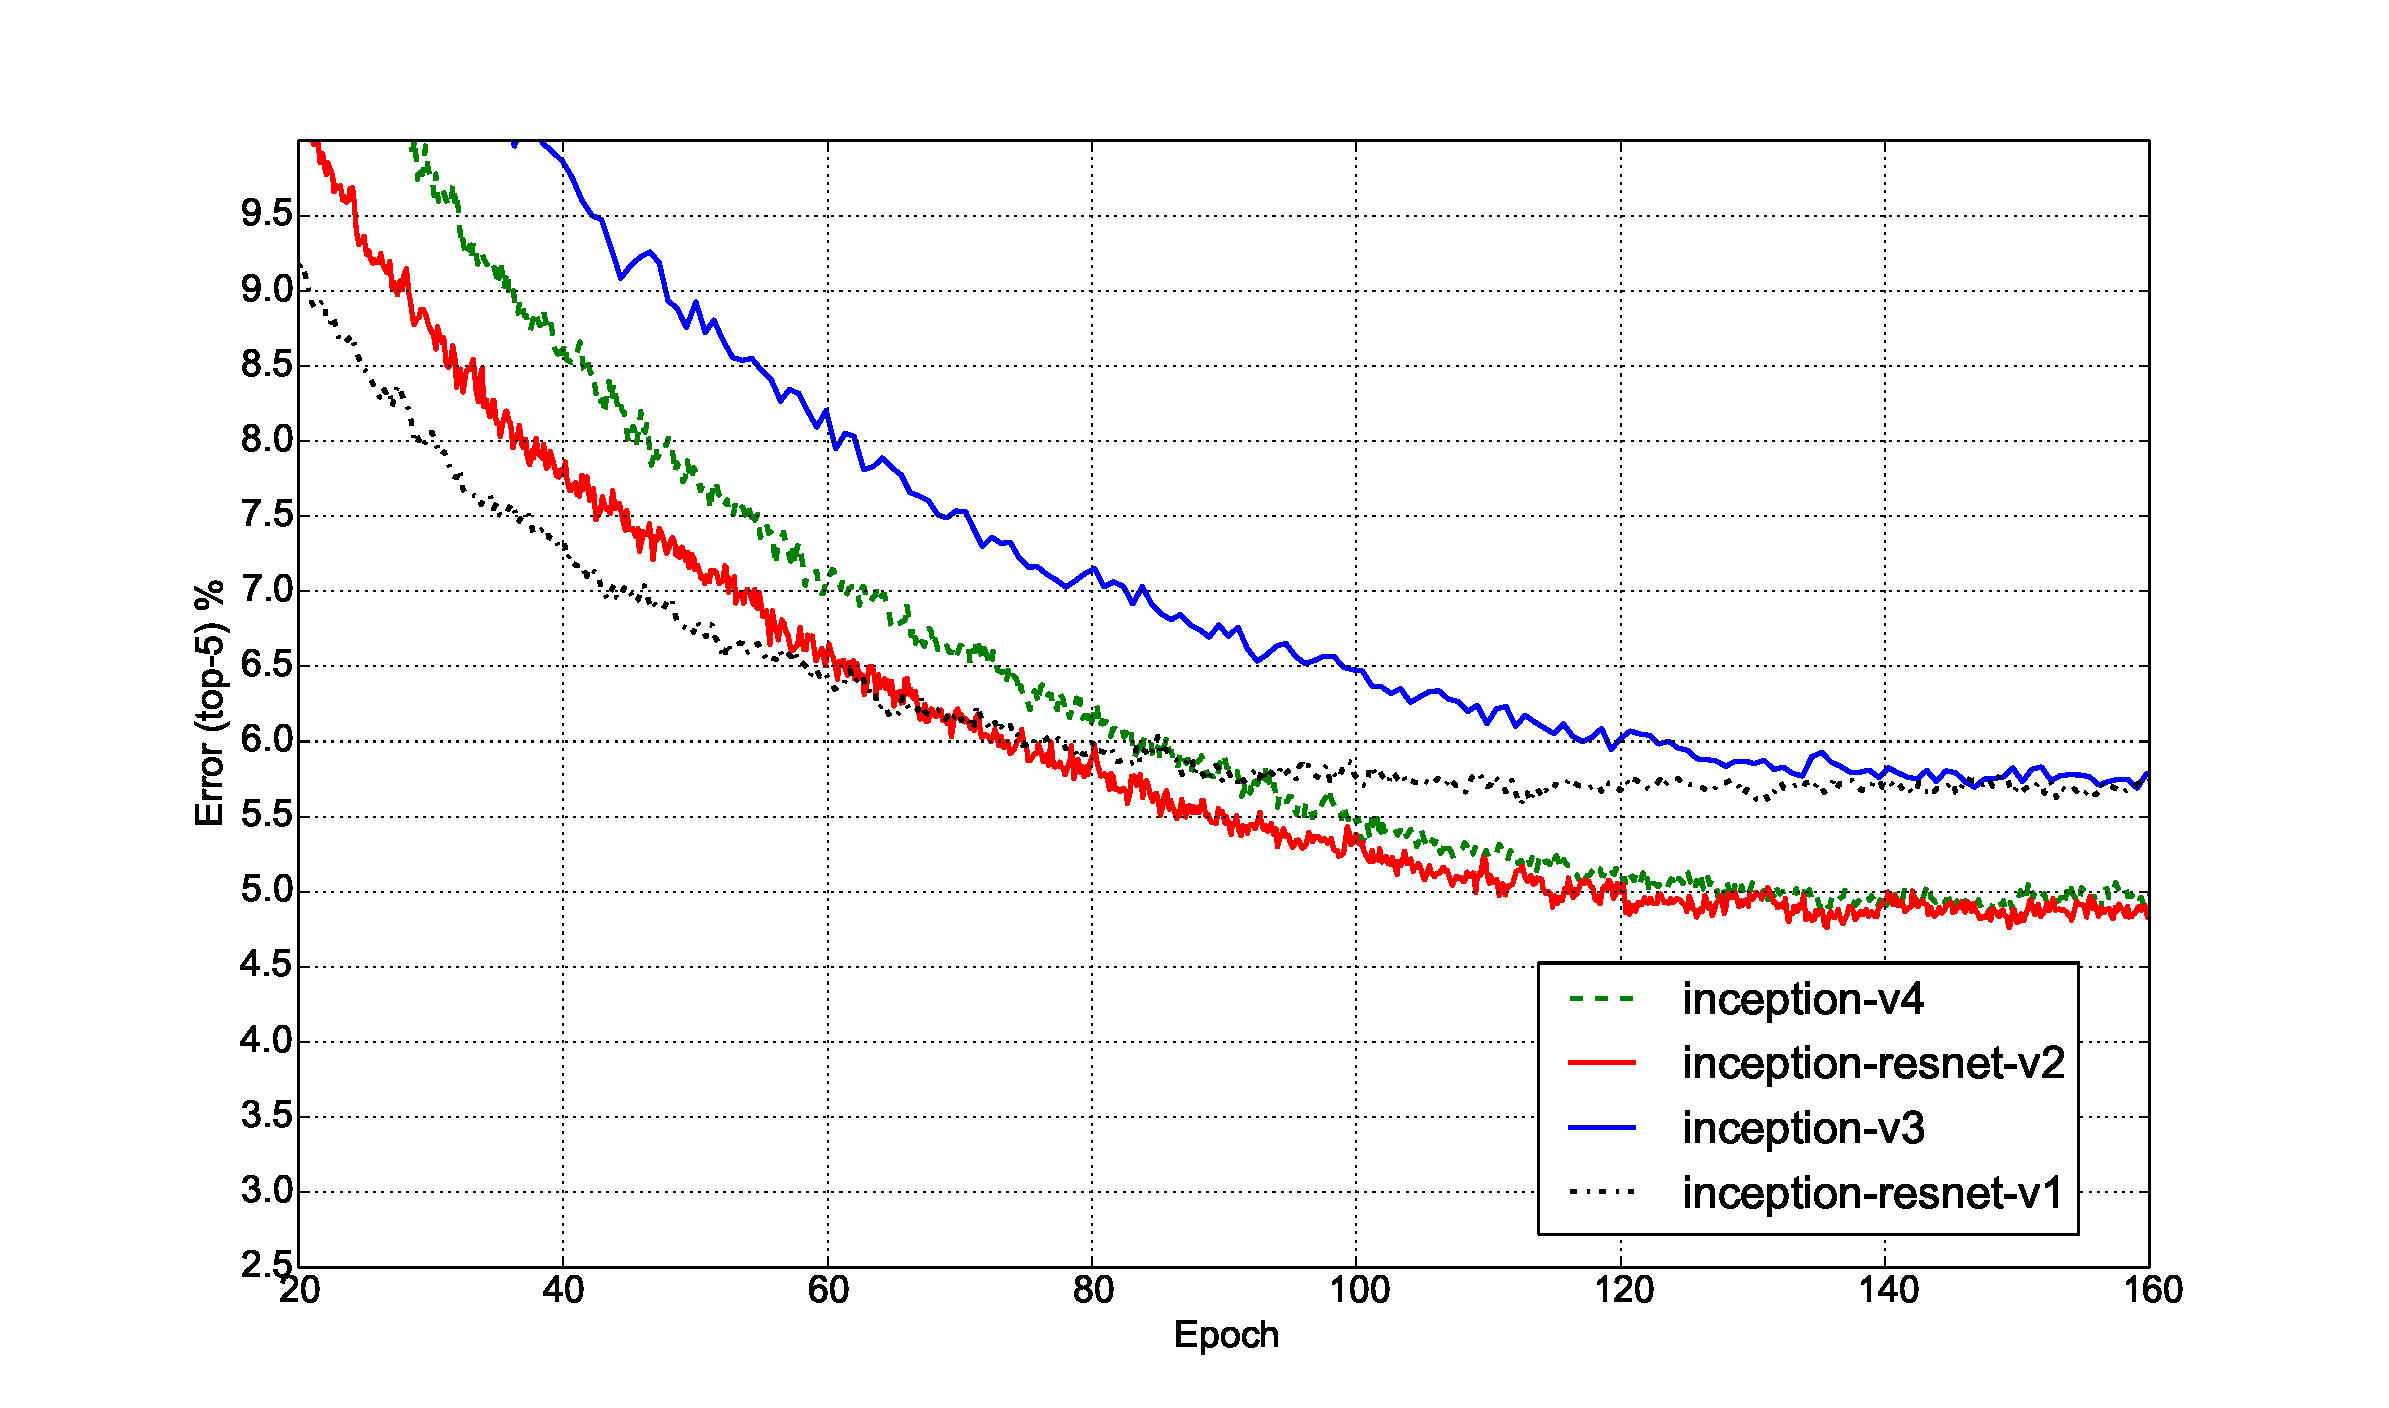
\includegraphics[width=\linewidth]{all_top5}
\caption{Top-5 error evolution of all four models (single model, single crop).
  Showing the improvement due to larger model size. Although the residual
  version converges faster, the final accuracy seems to mainly depend on the
  model size.
}
\label{fig:alltop5}
\end{figure}

\begin{figure}
\centering
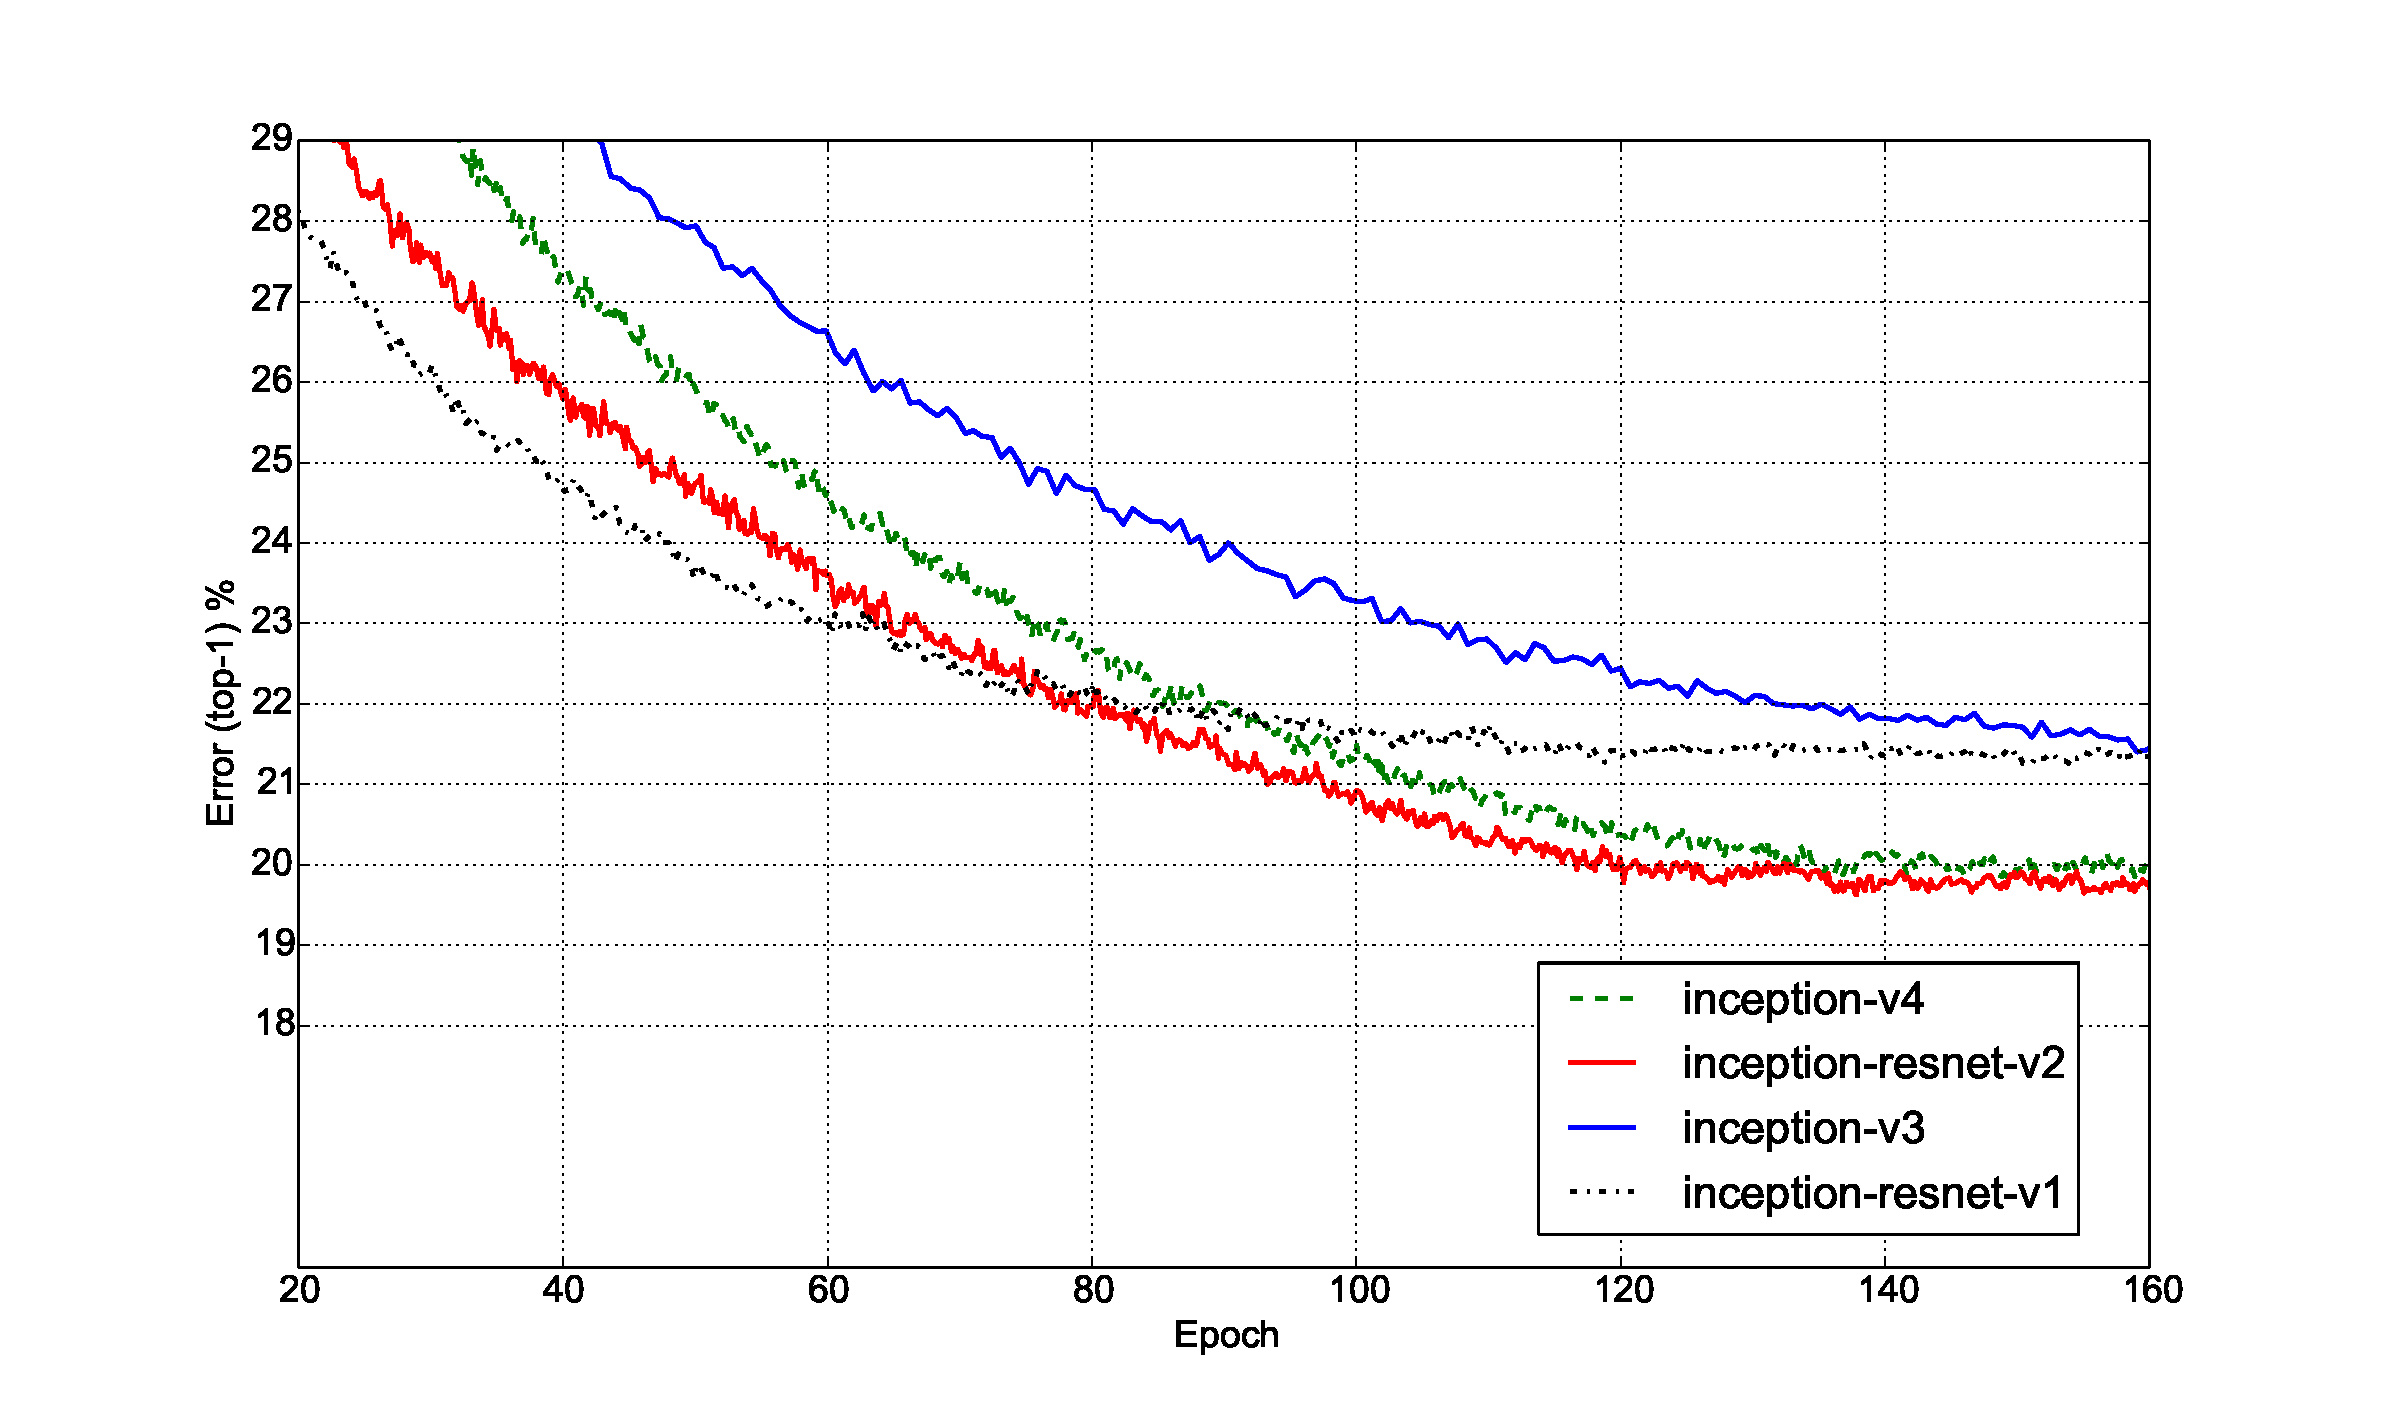
\includegraphics[width=\linewidth]{all_top1}
\caption{Top-1 error evolution of all four models (single model, single crop).
  This paints a similar picture as the top-5 evaluation.
}
\label{fig:alltop1}
\end{figure}

Finally, we present some comparisons, between various versions of Inception
and Inception-ResNet. The models Inception-v3 and Inception-v4 are deep
convolutional networks not utilizing residual connections while
Inception-ResNet-v1 and Inception-ResNet-v2 are Inception style networks
that utilize residual connections instead of filter concatenation.

\begin{table}
{\small
 \begin{center}
   \begin{tabular}[H]{|l|c|c|}
   \hline
   {\bf Network} & {\bf Top-1 Error} & {\bf Top-5 Error} \\
   \hline
   BN-Inception~\cite{ioffe2015batch} & 25.2\% & 7.8\% \\
   Inception-v3~\cite{szegedy2015rethinking} & 21.2\% & 5.6\% \\
   Inception-ResNet-v1 & 21.3\% & 5.5\% \\
   Inception-v4 & 20.0\% & 5.0\% \\
   Inception-ResNet-v2 & 19.9\% & 4.9\% \\
   \hline
   \end{tabular}
 \end{center}
 }
\caption{Single crop - single model experimental results. Reported on the
non-blacklisted subset of the validation set of ILSVRC 2012.}
\label{singlesingle}
\end{table}
\begin{table}
{\small
 \begin{center}
   \begin{tabular}[H]{|l|c|c|c|}
   \hline
   {\bf Network} & {Crops} & {\bf Top-1 Error} & {\bf Top-5 Error} \\
   \hline
   ResNet-151~\cite{he2015deep} & 10 & 21.4\% & 5.7\% \\
   Inception-v3~\cite{szegedy2015rethinking} & 12 & 19.8\% & 4.6\% \\
   Inception-ResNet-v1 & 12 & 19.8\% & 4.6\% \\
   Inception-v4 & 12 & 18.7\% & 4.2\% \\
   Inception-ResNet-v2 & 12 & 18.7\% & 4.1\% \\
   \hline
   \end{tabular}
 \end{center}
 }
\caption{10/12 crops evaluations - single model experimental results.
  Reported on the
all 50000 images of the validation set of ILSVRC 2012.}
\label{multisingle}
\end{table}
\begin{table}
{\small
 \begin{center}
   \begin{tabular}[H]{|l|c|c|c|}
   \hline
   {\bf Network} & {Crops} & {\bf Top-1 Error} & {\bf Top-5 Error} \\
   \hline
   ResNet-151~\cite{he2015deep} & dense & 19.4\% & 4.5\% \\
   Inception-v3~\cite{szegedy2015rethinking} & 144 & 18.9\% & 4.3\% \\
   Inception-ResNet-v1 & 144 & 18.8\% & 4.3\% \\
   Inception-v4 & 144 & 17.7\% & 3.8\% \\
   Inception-ResNet-v2 & 144 & 17.8\% & 3.7\% \\
   \hline
   \end{tabular}
 \end{center}
 }
\caption{144 crops evaluations - single model experimental results.
  Reported on the all 50000 images of the validation set of ILSVRC 2012.}
\label{manysingle}
\end{table}
\begin{table}
{\small
 \begin{center}
   \begin{tabular}[H]{|l|c|c|c|}
   \hline
   {\bf Network} & {Models} & {\bf Top-1 Error} & {\bf Top-5 Error} \\
   \hline
   ResNet-151~\cite{he2015deep} & 6 & -- & 3.6\% \\
   Inception-v3~\cite{szegedy2015rethinking} & 4 & 17.3\% & 3.6\% \\
   \stackanchor{Inception-v4 + }{$3\times$ Inception-ResNet-v2} & 4 &
   16.5\% & 3.1\% \\
   \hline
   \end{tabular}
 \end{center}
 }
\caption{Ensemble results with 144 crops/dense evaluation.
  Reported on the all 50000 images of the validation set of ILSVRC 2012.
  For Inception-v4(+Residual), the ensemble consists of one pure Inception-v4
  and three Inception-ResNet-v2 models and were evaluated both on the
  validation and on the test-set. The test-set performance was
  $3.08\%$ top-5 error verifying that we don't over-fit on the validation
  set.
}
\label{manyensemble}
\end{table}

Table~\ref{singlesingle} shows the single-model, single crop top-1 and
top-5 error of the various architectures on the validation set.

Table~\ref{multisingle} shows the performance of the various models with a
small number of crops: 10 crops for ResNet as was reported
in~\cite{he2015deep}), for the Inception variants, we have used the 12 crops
evaluation as as described in~\cite{szegedy2015going}.

Table~\ref{manysingle} shows the single model performance of the various
models using. For residual network the dense evaluation result is reported
from~\cite{he2015deep}. For the inception networks, the 144 crops strategy
was used as described in~\cite{szegedy2015going}.

Table~\ref{manyensemble} compares ensemble results. For the pure residual
network the 6 models dense evaluation result is reported
from~\cite{he2015deep}. For the inception networks 4 models were ensembled
using the 144 crops strategy as described in~\cite{szegedy2015going}.
